\lesson{12}{29.11.2023}{АВЛ-дерево, хэширование, B-деревья}

\chapter{Информационный поиск и организация информации}

\section{АВЛ-дерево}

\begin{definition}
    Высота дерева --- длина пути (количество ребер) от корня до листьев.\\
    Вершина дерева называется сбалансированной, если высоты ее правого и левого поддеревьев различаются не более чем на 1.\\
    Двоичное дерево называется сбалансированным, если каждая его вершина сбалансирована.\\
    Чтобы при добавлении элементов в дерево время поиска росло не слишком быстро, его нужно балансировать.\\
    АВЛ-дерево (самобалансирующееся дерево) позволяет поддерживать приблизительное равенство двух ветвей двоичного дерева во всех его узлах, затрагивая за раз не более трех из них.
\end{definition}

\begin{algoritm}(Балансировка)
    
    \begin{enumerate}
        \item добавляем вершину $d$
        \item проверяем вершины на пути от $d$ к корню
        \item обозначим через $a, b, c$ ($b, c$ -- потомки $a$) первые несблансированные вершины на пути от $d$ к корню (баланс может нарушится только в трех или в двух вершинах)
        \item выполняем перебалансировку (поворот):
    \end{enumerate}


    \textbf{2 вида перебалансировки:}
    \begin{enumerate}
        \item узел $b$ "вытягиваем" вверх на место $a$, так, что $a$ становится потомком $b$ ($b$ соотвественно "прикрепляется" к узлу выше, если он был). Поддерево на $b$ становится поддеревом $a$.
        
        \begin{minipage}{0.45\textwidth}
            \begin{tikzpicture}[->,>=stealth, level/.style={sibling distance = 3.5cm/#1, level distance = 1.5cm}, scale=0.6,transform shape]
                \node [treenode] {$a$}
                child
                {
                    node [treenode] {$b$} 
                    child
                    {
                        node [treenode] {$c$} 
                        child[edge from parent path ={(\tikzparentnode.south) -- (\tikzchildnode.north)}]
                        {
                            node [subtree,yshift=0.4cm] (c) {}   % delay the text till later
                        }
                        child[edge from parent path ={(\tikzparentnode.south) -- (\tikzchildnode.north)}]
                        {
                            node [subtree,yshift=0.4cm] (d) {}       % delay the text till later
                        }
                    }
                    child[edge from parent path ={(\tikzparentnode.-50) -- (\tikzchildnode.north)}]
                    {
                        node [subtree,yshift=0.4cm] (a) {}   % delay the text till later
                    }
                }
                child[edge from parent path ={(\tikzparentnode.-30) -- (\tikzchildnode.north)}]
                {
                    node [subtree,yshift=0.4cm] (b) {}       % delay the text till later
                }
            ;
            % ------------------------------------------------ put the text into subtree nodes
            \node[align=center,yshift=0.1cm] at (a) {$R$};
            \node[align=center,yshift=0.1cm] at (b) {$S$};
            \node[align=center,yshift=0.1cm] at (c) {$P$};
            \node[align=center,yshift=0.1cm] at (d) {$Q$};
            \end{tikzpicture}    
        \end{minipage} $\to$
        \begin{minipage}{0.45\textwidth}
            \begin{tikzpicture}[->,>=stealth, scale=0.6,transform shape]
                \node [treenode] (b) at (0,0) {$b$};
                \node [treenode] (c) at (-2,-2) {$c$};
                \node [treenode] (a) at (2,-2) {$a$};
                \node [subtree] (c1) at (-3,-4) {$P$};
                \node [subtree] (d) at (-1,-4) {$Q$};
                \node [subtree] (a1) at (1,-4) {$R$};
                \node [subtree] (b1) at (3,-4) {$S$};
                
                \draw (b) -- (c);
                \draw (b) -- (a);
                \draw (c) -- (c1);
                \draw (c) -- (d);
                \draw (a) -- (a1);
                \draw (a) -- (b1);
            \end{tikzpicture}    
        \end{minipage}
    
    \item узел $c$ "вытягиваем" вверх, $a$ -- левый ребенок, $b$ -- правый ребенок. Левое поддерево $c$ прикрепляется к $a$, правое -- к $b$.
    
    
    \begin{minipage}{0.45\textwidth}    
        \begin{tikzpicture}[->,>=stealth, level/.style={sibling distance = 3.5cm/#1, level distance = 1.5cm}, scale=0.6,transform shape]
            \node [treenode] {$a$}
            child[edge from parent path ={(\tikzparentnode.west) -- (\tikzchildnode.north)}]
            {
                node [subtree,yshift=0.4cm] (b) {}       % delay the text till later
            }
            child
            {
                node [treenode] {$b$} 
                child
                {
                    node [treenode] {$c$} 
                    child[edge from parent path ={(\tikzparentnode.south) -- (\tikzchildnode.north)}]
                    {
                        node [subtree,yshift=0.4cm] (c) {}   % delay the text till later
                    }
                    child[edge from parent path ={(\tikzparentnode.south) -- (\tikzchildnode.north)}]
                    {
                        node [subtree,yshift=0.4cm] (d) {}       % delay the text till later
                    }
                }
                child[edge from parent path ={(\tikzparentnode.-50) -- (\tikzchildnode.north)}]
                {
                    node [subtree,yshift=0.4cm] (a) {}   % delay the text till later
                }
            }
            
        ;
        % ------------------------------------------------ put the text into subtree nodes
        \node[align=center,yshift=0.1cm] at (a) {$S$};
        \node[align=center,yshift=0.1cm] at (b) {$R$};
        \node[align=center,yshift=0.1cm] at (c) {$P$};
        \node[align=center,yshift=0.1cm] at (d) {$Q$};
        \end{tikzpicture}
    \end{minipage} $\to$
    \begin{minipage}{0.45\textwidth}
        \begin{tikzpicture}[->,>=stealth, scale=0.6,transform shape]
            \node [treenode] (b) at (0,0) {$c$};
            \node [treenode] (c) at (-2,-2) {$a$};
            \node [treenode] (a) at (2,-2) {$b$};
            \node [subtree] (c1) at (-3,-4) {$P$};
            \node [subtree] (d) at (-1,-4) {$Q$};
            \node [subtree] (a1) at (1,-4) {$R$};
            \node [subtree] (b1) at (3,-4) {$S$};
            
            \draw (b) -- (c);
            \draw (b) -- (a);
            \draw (c) -- (c1);
            \draw (c) -- (d);
            \draw (a) -- (a1);
            \draw (a) -- (b1);
        \end{tikzpicture}
    \end{minipage}
    \end{enumerate}
\end{algoritm}


\begin{theorem}
    После операции поворота полученное дерево окажется сбалансированным.
\end{theorem}

\begin{proof}(да, я просто списал с Романовского :с)
    Обозначим за $H(i$$)$ максимальную длину пути от добавленной вершины до вершины $i$, за $h_k$ - максимальную высоту поддерева $K$.

    По предположению: 
    $$H(a) = H(b) + 1 = H(c) + 2,$$ 
    $$h_s = H(b) - 2 = H(c) - 1$$

    Рассмотрим отдельно 2 случая:
    \begin{enumerate}
        \item  $h_R < H(c)$.  Тогда после первой балансировки дерева  $H(a) = h_s + 1 = H(c)$ и высота верхней вершины стала меньше
        \item в этом случае высота так же уменьшается на 1, так как определяющие максимальный путь поддеревья R и Q поднялись на одну ступень выше.
    \end{enumerate}
\end{proof}

\section{Хэширование}

\begin{definition}
    Хеш — это функция, сопоставляющая объектам какого-то множества числовые значения из ограниченного промежутка.

    «Хорошая» хеш-функция:
    \begin{itemize}
        \item Быстро считается — за линейное от размера объекта время;
        \item Имеет не очень большие значения — влезающие в 64 бита;
        \item «Детерминировано-случайная» — если хеш может принимать $n$ различных значений, то вероятность того, что хеши от двух случайных объектов совпадут, равна примерно $\frac{1}{n}$.
    \end{itemize}

    Обычно хеш-функция не является взаимно однозначной: одному хешу может соответствовать много объектов, т.е. она сюръективная.
\end{definition}

$\newline$

Пример:
\begin{figure}[H]
    \centering
    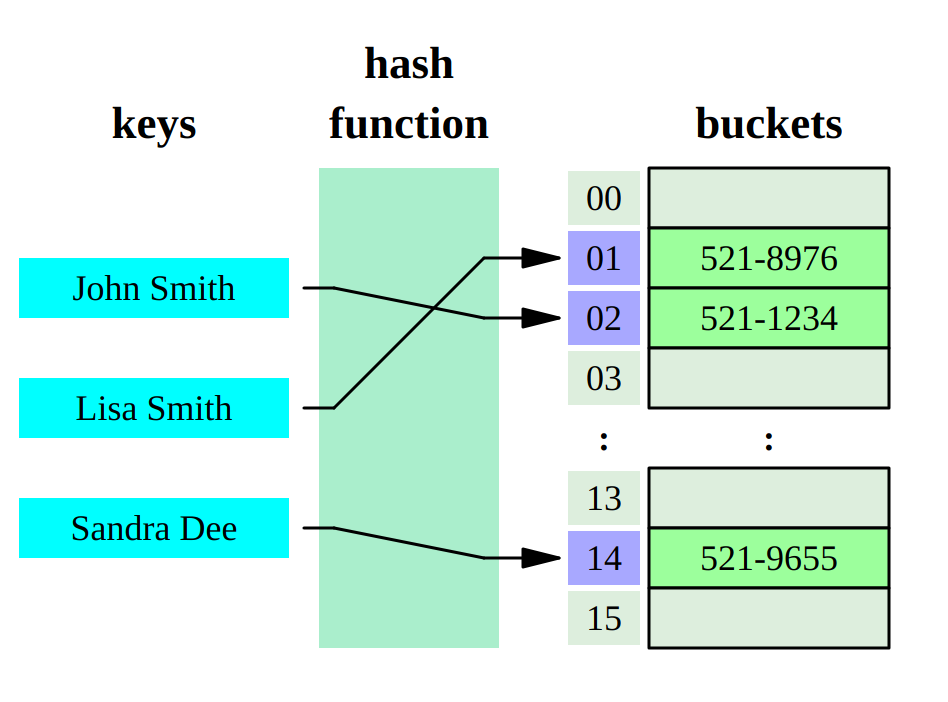
\includegraphics[width=\linewidth]{kakoi-map-bystree-i-est-li-alternativa-Judy-2.png}
\end{figure}


\section{B-деревья}

\begin{definition}
    B-дерево --- сильноветвящееся сбалансированное дерево поиска, в котором каждый узел содержит множество ключей и имеет более двух потомков.

    Элементы находятся в листьях, остальные уровни представляют собой иерархию индексов, они указывают путь, по какой ветке двигаться, чтобы прийти в тот лист, где находится нужная запись.

    Количество ключей в узле и количество потомков зависит от порядка B-дерева. Для каждого дерева фиксируется какое-то число $t$.

    B-дерево обладает следующими свойствами:
    \begin{enumerate}
        \item Все листья находятся на одном и том же уровне, т.е. имеют одинаковую глубину (B-дерево идеально сбалансировано)
        \item Каждый узел, кроме корневого, должен иметь, как минимум $t-1$, и не более $2t-1$ ключей
        \item Если узел не является листом, то он имеет детей (кол-во ключей в узле + 1) штук
        \item Все ключи в узле должны располагаться в порядке возрастания их значений
    \end{enumerate}
\end{definition}

\begin{remark}
    Примеры для всех операций в B-дереве очень долго писать, можете потыкать \href{https://www.cs.usfca.edu/~galles/visualization/BTree.html}{тут} (открывайте в pdf)
\end{remark}

\begin{algoritm}(Поиск в B-дереве)
    \begin{enumerate}
        \item Считать элемент для поиска
        \item Сравнить искомый элемент с первым значением ключа в корневом узле дерева.
        \item Если они совпадают, вернуть значение.
        \item Если они не совпадают, проверить больше или меньше значение элемента, чем текущее значение ключа.
        \item Если искомый элемент меньше, продолжить поиск по левому поддереву.
        \item Если искомый элемент больше, сравнить элемент со следующим значением ключа в узле и повторять Шаги 3, 4, 5 и 6 пока не будет найдено совпадение или пока искомый элемент не будет сравнен с последним значением ключа в узле-листе.
        \item Если последнее значение ключа в узле-листе не совпало с искомым, вернуть $null$.
    \end{enumerate}
\end{algoritm}


\begin{algoritm}(Добавление элемента)
    В В-дереве новый элемент может быть добавлен только в узел-лист. Вставка происходит следующим образом:
    \begin{enumerate}
        \item Проверить пустое ли дерево.
        \item Если дерево пустое, создать новый узел с новым значением ключа и его принять за корневой узел.
        \item Если дерево не пустое, найти подходящий узел-лист, к которому будет добавлено новое значение, используя логику дерева двоичного поиска.
        \item Если в текущем узле-листе есть незанятая ячейка, добавить новый ключ-значение к текущему узлу-листу, следуя возрастающему порядку значений ключей внутри узла.
        \item Если текущий узел полон и не имеет свободных ячеек, разделите узел-лист, отправив среднее значение родительскому узлу. Повторяйте шаг, пока отправляемое значение не будет зафиксировано в узле.
        \item Если разделение происходит с корнем дерева, тогда среднее значение становится новым корнем дерева и высота дерева увеличивается на единицу.
    \end{enumerate}
\end{algoritm}

\begin{algoritm}(Удаление элемента)
    \begin{enumerate}
        \item Если корень является листом (в дереве только один узел), просто удаляем ключ из этого узла.
        \item Находим узел $x$, содержащий ключ, запоминая путь к нему.
        \item  Если $x$ — лист, удаляем ключ из $x$.
        Если в $x$ осталось не меньше $t-1$ ключей, процедура завершается.
        \item Если соседний правый узел имеет не менее $t$ ключей, переносим ключ-разделитель в $x$ и первый ключ соседа на место разделителя. Если соседний правый узел не подходит, но соседний левый узел имеет не менее $t$ ключей, аналогично переносим ключ-разделитель и последний ключ соседа.
        Если ни один из соседей не подходит, объединяем $x$ с одним из соседей и перемещаем разделяющий ключ в объединенный узел.
        \item Если после объединения в родительском узле остается $t-2$ ключей и это не корень, повторяем процедуру для родителя.
        \item Если в результате в корне осталось от $1$ до $t-1$ ключей, дополнительных действий не требуется.
        Если в корне не осталось ключей, исключаем корневой узел и делаем его единственного потомка новым корнем дерева.
        \item Если $x$ не является листом, удаляем самый правый ключ из поддерева $i$-го потомка $x$ или самый левый ключ из поддерева $(i+1)$-го потомка x. Заменяем удаленный ключ на место ключа $K$.
    \end{enumerate}
\end{algoritm}